\chapter{Números complejos}
\unsection{Introducción}
Este es el primer tema de la materia, los números complejos nos van ayudar en el análisis de señales y sistemas por ende es de vital importancia entenderlos plenamente.
La unidad compleja se define como:
\begin{equation}\label{eq:j}
    i=\sqrt{-1}
\end{equation}{}
De esta definición podemos intuir que:
\begin{equation}\label{eq:jj}
    i^2=-1 \lrah \sqrt{-1}\cdot\sqrt{-1}=-1 
\end{equation}{}
Ahora bien, todo estudiante de ingeniería electrónica sabe que $i$ es por corriente asi que para los propositos de este curso usaremos $j$ en vez de $i$ 
\unsection{Números complejos}
Un numero complejo se puede interpretar como un vector de 2 dimensiones conformado por 2 partes, la parte real y la parte imaginaria. La unidad de la parte imaginaria sera $j$ y la unidad de la parte real sera el $1$, escalando (multiplicando por un escalar) y sumando estas 2 unidades seremos capaz de representar cualquier numero complejo, por lo tanto estas dos unidades son la base de un espacio vectorial ya que cualquier numero complejo, que es un vector, se puede expresar como la suma de estos 2 versores:
\begin{equation}\label{eq:cart}
    z=u\cdot(1,j0)+v\cdot (0,j1)
\end{equation}
Siendo $u$ y $v$ números reales.
\begin{figure}[H]
    \centering
         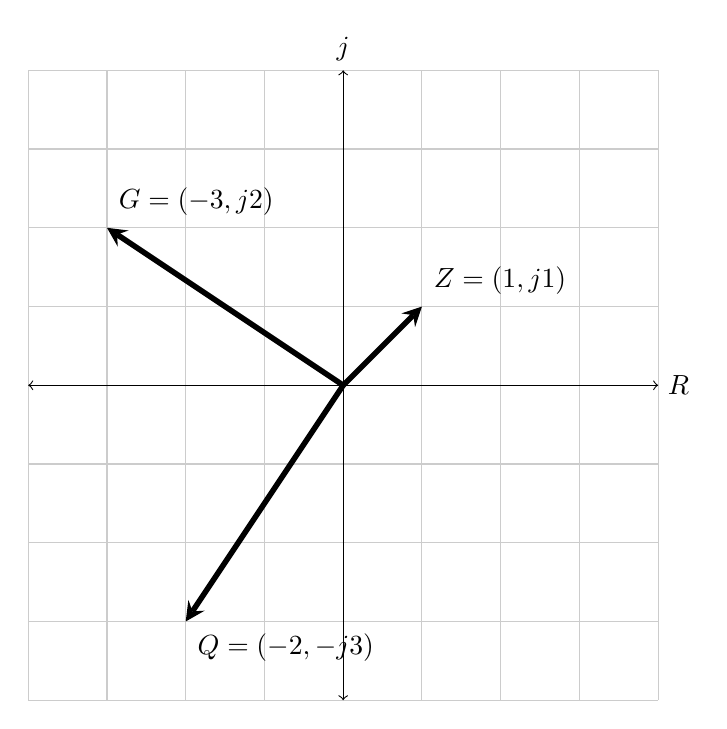
\begin{tikzpicture}
        \draw[thin,gray!40] (-4,-4) grid (4,4);
        \draw[<->] (-4,0)--(4,0) node[right] {$R$};
        \draw[<->] (0,-4)--(0,4) node[above]{$j$};
        \draw[line width=2pt,black,-stealth](0,0)--(1,1) node[anchor=south west]{${Z=(1,j1)}$};
        \draw[line width=2pt,black,-stealth](0,0)--(-3,2) node[anchor=south west]{${G=(-3,j2)}$};
        \draw[line width=2pt,black,-stealth](0,0)--(-2,-3) node[anchor=north west]{${Q=(-2,-j3)}$};
    \end{tikzpicture}
    \caption{Ejemplo de representacion de numero en el plano complejo}
    \label{fig:EjmNc}
\end{figure}
Como se puede intuir en al figura\ref{fig:EjmNc} acada punto del plano complejo le corresponde un valor imaginario y uno complejo, formando un espacio vectorial. También se pude apreciar que ambas unidades forman una base ortonormal.

Al ser el numero complejo un vector se puede escribir de distintas formas. La forma mas familiar de representar un numero complejo, para este punto sera de la forma cartesiana. Comparando un numero en el plano complejo y un vector en el plano de 2 dimensiones reales se puede apreciar la similitud.

\begin{figure}[H]%
\centering
    \begin{minipage}{0.5\textwidth}
    \centering
        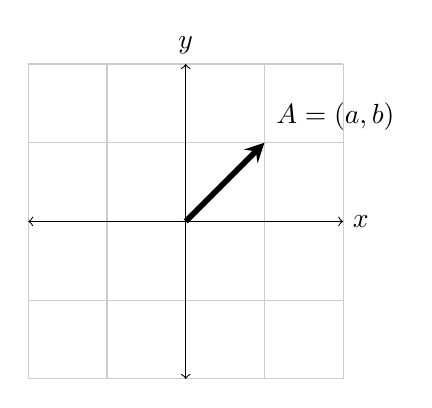
\begin{tikzpicture}
    \draw[thin,gray!40] (-2,-2) grid (2,2);
    \draw[<->] (-2,0)--(2,0) node[right] {$x$};
    \draw[<->] (0,-2)--(0,2) node[above]{$y$};
    \draw[line width=2pt,black,-stealth](0,0)--(1,1) node[anchor=south west]{${A=(a,b)}$};
\end{tikzpicture}
\caption*{$A=\hat{x}\cdot a+\hat{y}\cdot b$}
    \end{minipage}%
    \begin{minipage}{0.4\textwidth}
    \centering
        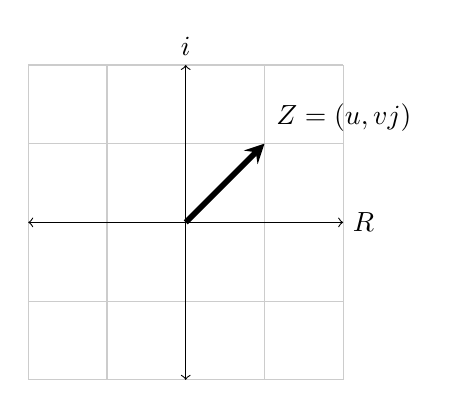
\begin{tikzpicture}
        \draw[thin,gray!40] (-2,-2) grid (2,2);
        \draw[<->] (-2,0)--(2,0) node[right] {$R$};
        \draw[<->] (0,-2)--(0,2) node[above]{$i$};
        \draw[line width=2pt,black,-stealth](0,0)--(1,1) node[anchor=south west]{${Z=(u,vj)}$};
\end{tikzpicture}
\caption*{$Z=u+j\cdot v$}
    \label{fig:test2}
    \end{minipage}%
    \caption{Comparación entre un numero complejo y un vector de 2 dimensiones reales}
    \label{fig:compri}
\end{figure}
En la figura:\ref{fig:compri} se muestra un vector real de 2 dimensiones $A$, compuesto por 2 componentes $a$ y $b$ ambos componentes están multiplicando a un versor de la base ($\hat{x}\ ,\ \hat{y}$). De manera similar también se muestra un numero complejo $Z$ el cual esta conformado por $u$ y $v$, $\ u$ siendo la parte real y $\ v$ siendo la parte imaginaria, ya que $\ v$ esta multiplicando la unidad imaginaria.
Las otras representaciones de un numero complejo son la forma polar y la forma exponencial.
\unsubsection{Forma polar}
La forma polar de un numero complejo tiene por datos el ángulo con respecto a el eje real (por convención), comúnmente llamado argumento y el modulo del numero complejo. Plateando un numero complejo de la forma:
\begin{equation}\label{eq:polz}
    z=x+jy
\end{equation}
\begin{figure}[H]
    \centering
        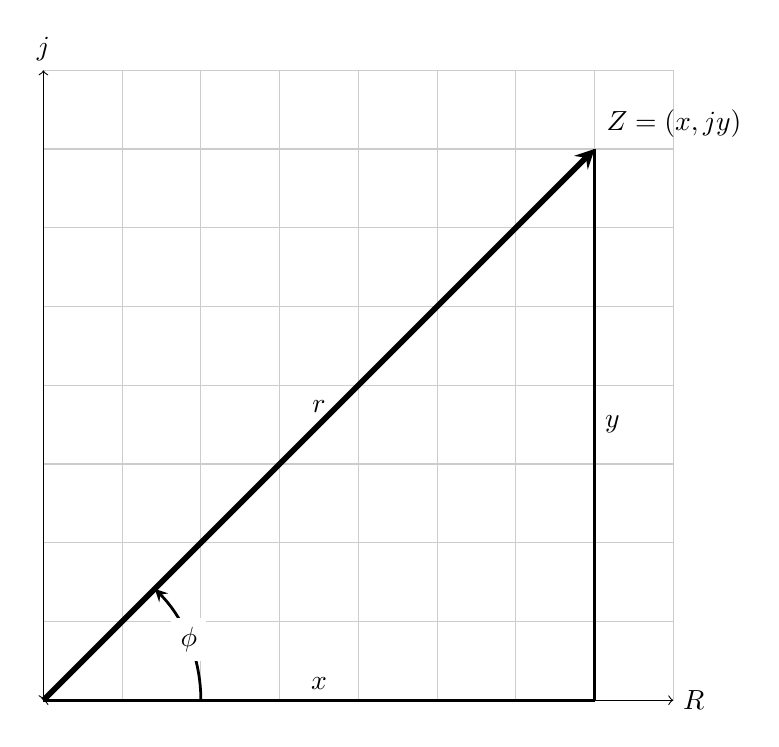
\begin{tikzpicture}
        \draw[thin,gray!40] (0,0) grid (8,8);
        \draw[<->] (0,0)--(8,0) node[right] {$R$};
        \draw[<->] (0,0)--(0,8) node[above]{$j$};
        \draw[line width=2pt,black,-stealth](0,0)--node[above]{$r$}(7,7) node[anchor=south west]{${Z=(x,jy)}$};
        \draw[line width=1pt,black,-](7,0)-- node[right]{$y$} (7,7);
        \draw[line width=1pt,black,-](0,0)-- node[above]{$x$}(7,0);
        \draw[line width=1pt,black,-stealth] (2,0) arc (0:45:2) node [midway,fill=white]{$\phi$};
\end{tikzpicture}
\caption{Planteo para la definición de la forma polar}
    \label{fig:Polar}
\end{figure}
Tomando en cuenta lo mostrado en la figura\ref{fig:Polar} podemos deducir que el modulo de un numero complejo es
\begin{equation}\label{eq:polr}
    r=\sqrt{x^2+y^2}
\end{equation}
Y además:
\begin{equation}\label{eq:polt}
    \phi=\arctan{(\dfrac{y}{x})}
\end{equation}
Por lo tanto:
\begin{equation}\label{eq:polx}
    x=r\cdot\cos{(\phi)}
\end{equation}
\begin{equation}\label{eq:poly}
    y=r\cdot\sin{(\phi)}
\end{equation}
Y por ultimo remplazndo \ref{eq:polx} y \ref{eq:poly} en \ref{eq:polz} obtenemos la forma final de un numero complejo en su forma polar:
\begin{equation}\label{eq:defPol}
    z=x+yj \llrah \ z=r\cdot[\cos{(\phi)}+j\sen{(\phi)}]
\end{equation}
Esta ecuación nos deja al descubierto una propiedad muy interesante de los números complejos. Al estar la forma polar definida a partir de cosenos y senos nos da a entender que varios números complejo de mismo modulo y distinto argumento pueden ser iguales, ya que el seno y el coseno son funciones periódicas en $2\pi$. 
\begin{figure}[H]%
\centering
    \begin{minipage}{0.5\textwidth}
    \centering
        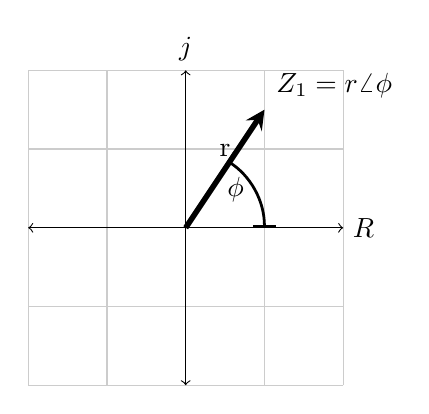
\begin{tikzpicture}
        \draw[thin,gray!40] (-2,-2) grid (2,2);
        \draw[<->] (-2,0)--(2,0) node[right] {$R$};
        \draw[<->] (0,-2)--(0,2) node[above]{$j$};
        \draw[line width=2pt,black,-stealth](0,0)--node[above]{r}(1,1.5) node[anchor=south west]{$Z_1=r\angle{\phi}$};
        \draw[line width=1pt,black,|-|] (1,0) arc (0:58:1) node [midway, left]{$\phi$};
    \end{tikzpicture}
    \end{minipage}%
    \begin{minipage}{0.4\textwidth}
    \centering
       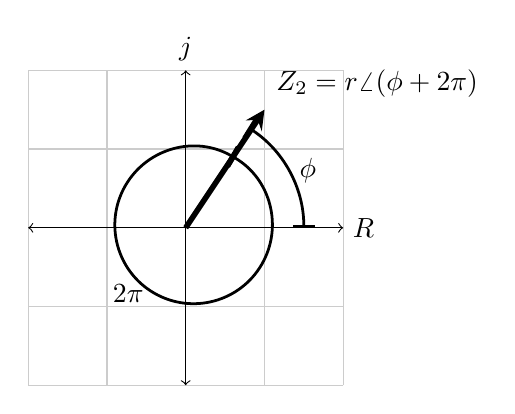
\begin{tikzpicture}
        \draw[thin,gray!40] (-2,-2) grid (2,2);
        \draw[<->] (-2,0)--(2,0) node[right] {$R$};
        \draw[<->] (0,-2)--(0,2) node[above]{$j$};
        \draw[line width=2pt,black,-stealth](0,0)--node[above]{}(1,1.5) node[anchor=south west]{$Z_2=r\angle{(\phi+2\pi)}$};
        \draw[line width=1pt,black,|-|] (0.6,0.902) arc (60:420:1) node [midway, left]{$2\pi$};
        \draw[line width=1pt,black,|-|] (1.5,0) arc (0:58:1.5) node [midway, right]{$\phi$};
    \end{tikzpicture}
    \label{fig:Perz}
    \end{minipage}%
    \caption{Comparación entre números complejos de igual modulo y argumentos $\phi_1$ y $\phi_2=2\pi+\phi_1$}
    \label{fig:Perio}
\end{figure}
\begin{figure}[H]
\centering
    \pgfplotsset{compat = newest}
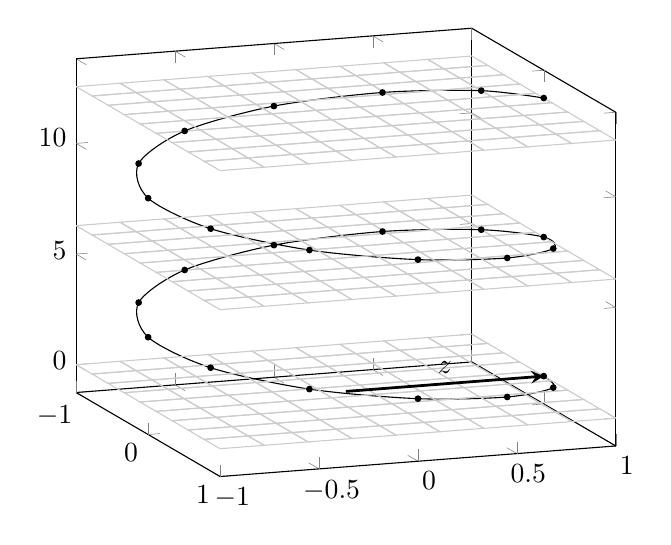
\begin{tikzpicture}
\begin{axis}[view={70}{15}]
    \addplot3+ [mark options={scale=0.5,fill=black,draw=black,},smooth,black,domain=0:4*pi,samples y=0] ({sin(deg(x))},{cos(deg(x))},{x});
    \addplot3+ [thin,no markers,mesh,draw=gray!40,domain=-1:1,samples=10] {2*pi};
    \addplot3+ [thin,no markers,mesh,draw=gray!40,domain=-1:1,samples=10] {0};
    \addplot3+ [thin,no markers,mesh,draw=gray!40,domain=-1:1,samples=10] {4*pi};
    \draw [line width=1pt,black,-stealth](0,0,0)--(0,1,0) node[midway, above]{$z$};
\end{axis}
\end{tikzpicture}
\caption{Representación de un numero $z=1[\cos{(\phi)}+j\sen{(\phi)}]$ siendo $\phi$ una variable correspondiente al eje $z$.}

    \label{fig:PerioC3}
\end{figure}
En la figura \ref{fig:PerioC3} se muestra un numero complejo al que se le modifica el argumento expresado en eje $z$, modificando sus coordenadas $(x,jy)$. Cuando el eje $z=2\pi$ se puede apreciar como el numero complejo toma las mismas coordenadas $(x,jy)$ que cuando $z=0$, lo mismo cuando $z=4\pi$.  
Por esta razón se debe restringir los valores que puede tomar el argumento en un intervalo de modulo $2\pi$, ya que otros argumentos que se salgan fuera de el intervalo definido pueden ser representados dentro del mismo intervalo. Nos quedaremos con la notación recomendada por la cátedra, la cual indica que el argumento esta restringido en $-\pi<\phi\leq\pi$
\begin{figure}[H]
    \centering
        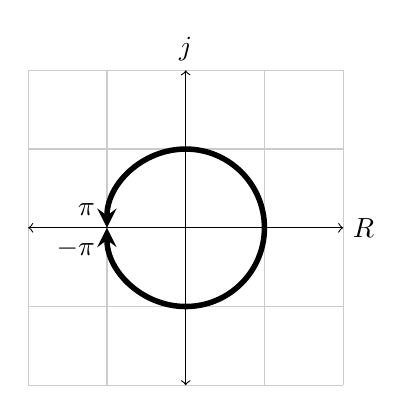
\begin{tikzpicture}
        \draw[thin,gray!40] (-2,-2) grid (2,2);
        \draw[<->] (-2,0)--(2,0) node[right] {$R$};
        \draw[<->] (0,-2)--(0,2) node[above]{$j$};
        \draw[line width=2pt,black,-stealth] (1,0) arc (0:180:1) node [anchor=south east]{$\pi$};
        \draw[line width=2pt,black,-stealth] (1,0) arc (0:-180:1) node [anchor=north east]{$-\pi$};
    \end{tikzpicture}
    \caption{Intervalo del argumento}
    \label{fig:interphi}
\end{figure}
\unsubsection{Forma exponencial}
Ser capaces de representar un numero complejo en su forma exponencial va a probar ser una de las herramientas más útiles de la materia. Para poder expresar un numero complejo en su forma exponencial se debe presentar las identidades trigonométricas definidas por las identidades de Euler, las cuales solo van a ser presentadas y no demostradas.
Las identidades trigonométricas son:
\begin{equation}\label{eq:eulers}
    \sin{(x)}=\cfrac{1}{2j}\cdot(e^{j\phi}-e^{-j\phi})
\end{equation}
\begin{equation}\label{eq:eulerc}
    \cos{(x)}=\cfrac{1}{2}\cdot(e^{j\phi}+e^{-j\phi})
\end{equation}
Remplazando \ref{eq:eulers} y \ref{eq:eulerc} en la ecuación de la defunción de la forma polar \ref{eq:defPol} obtenemos:
\begin{equation}
\begin{aligned}
      z=r\cdot[\cos{(\phi)}+j\sen{(\phi)}] \quad\Longrightarrow\quad z&=r\cdot[(\cfrac{1}{2}\cdot(e^{j\phi}+e^{-j\phi})+\cfrac{\bcancel{j}}{2\bcancel{j}}\cdot(e^{j\phi}-e^{-j\phi})]\\
      &=r[\cfrac{1}{2}\cdot(e^{j\phi}+e^{j\phi}+\bcancel{e^{-j\phi}}-\bcancel{e^{-j\phi}}]\\
      &=r[\bcancel{\cfrac{1}{2}}\cdot \bcancel{2}e^{j\phi}]\\
\end{aligned}
\end{equation}
\begin{equation}\label{eq:defExp}
    z=re^{j\phi}
\end{equation}
De esta manera obtenemos la definición de la forma exponencial. Esta manera de explicarlo es un poco ambigua ya que deja muchas preguntas sin contestar, cada uno elige hasta donde seguir el conejo blanco.
\unsection{Operaciones básicas y propiedades}
\unsubsection{Suma} 
    El plano complejo sigue las normas de un espacio vectorial por lo tanto la suma se computa componente a componente, en nuestro caso al ser un espacio vectorial de 2 dimensiones la suma se define como:
        \begin{equation}\label{eq:sum}
          z_1+z_2 \Rightarrow (x_1\ ,\ jy_1)+(x_2\ ,\ jy_2)=(x_1+x_2\ ,\ jy_1+jy_2))\\
        \end{equation}
    \begin{figure}[H]
        \centering
        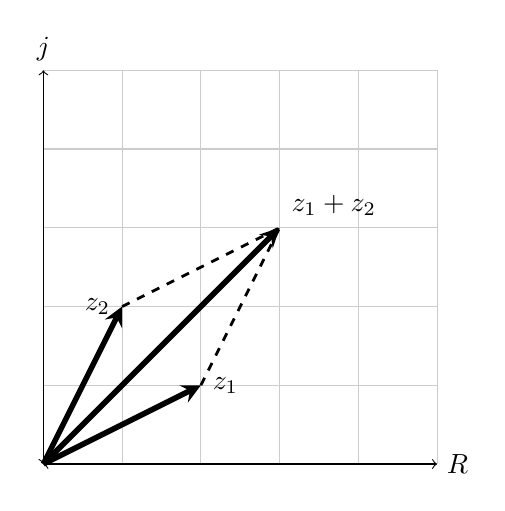
\begin{tikzpicture}
        \draw[thin,gray!40] (0,0) grid (5,5);
        \draw[<->] (0,0)--(5,0) node[right] {$R$};
        \draw[<->] (0,0)--(0,5) node[above]{$j$};
       \draw[line width=2pt,black,-stealth](0,0)--(1,2) node[left]{${z_2}$};
       \draw[line width=2pt,black,-stealth](0,0)--(2,1) node[right]{${z_1}$};
       \draw[line width=2pt,black,-stealth](0,0)--(3,3) node[anchor=south west]{${z_1+z_2}$};
       \draw[line width=1pt,black,dashed](1,2)--(3,3);
       \draw[line width=1pt,black,dashed](2,1)--(3,3);
    \end{tikzpicture}
    \caption{Representacion de la suma entre 2 numeros complejos}
        \label{fig:sumaC}
    \end{figure}
    Intuitivamente podemos apreciar que el elemento neutro de la suma es el vector $(0,0)$, por lo tanto el 0 en el plano complejo es el vector nulo.
        \begin{equation}\label{eq:sumnul}
            (x_1\ ,\ jy_1)+(0\ ,\ j0) \lrah (x_1+0\ ,\ jy_1+j0)=x_1+jy_1 \Rightarrow z_1+0 \\
        \end{equation}
    La suma hereda todas las propiedades de la suma en un espacio vectorial de $n$ dimensiones reales.
    \begin{itemize}
        \item Conmutatividad:
        \begin{equation}
            (a\ ,\ jb)+(\hat{a}\ ,\ j\hat{b})=(\hat{a}\ ,\ j\hat{b})+(a\ ,\ jb)
        \end{equation}
        \item Asociatividad:
        \begin{equation}
            [(a\ ,\ jb)+(\hat{a}\ ,\ j\hat{b})]+(\bar{a}\ ,\ j\bar{b})=(a\ ,\ jb)+[(\hat{a}\ ,\ j\hat{b})+(\bar{a}\ ,\ j\bar{b})]
        \end{equation}
        \item Elemento neutro:
        \begin{equation}
             (a\ ,\ jb)+(0\ ,\ j0) \lrah (a+0\ ,\ jb+j0)=a+jb 
        \end{equation}
        \item Opuesto (necesario para la resta):
        \begin{equation}
            -(a\ ,\ jb)=(-a\ ,\ -jb)
        \end{equation}
        Si sumamos a un $z$ su opuesto nos da como resultado el elemento neutro de la suma:
         \begin{equation}
            z-z=(a\ ,\ jb)-(a\ ,\ jb)\lrah \bcancel{(a-a)}+j\bcancel{(b-b)} = 0+j0
        \end{equation}
        Si restamos un $z_0=(x_0+jy_0)$ a un $z_1=(x_1+jy_1)$ obtendremos la expresión:
        \begin{equation}
            z_1-z_0=(x_1+jy_1)-(x_0+jy_0) \lrah z_0-z_1=(x_1-x_0)+j(y_1-y_0)
        \end{equation}
        \begin{figure}[H]
            \centering
            \begin{minipage}{0.4\textwidth}
            \centering
                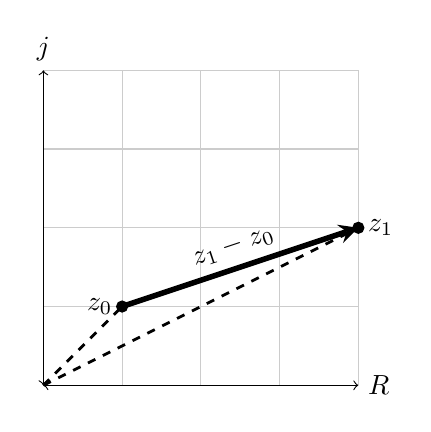
\begin{tikzpicture}
    \draw [thin,gray!40] (0,0) grid (4,4);
    \draw[<->] (0,0)--(4,0) node[right] {$R$};
    \draw[<->] (0,0)--(0,4) node[above]{$j$};
    \coordinate (a) at (1,1);
    \coordinate (b) at (4,2);
    \draw[fill=black] (a) circle(2pt) node[left]{$z_0$};
    \draw[fill=black] (b) circle(2pt) node[right]{$z_1$};
    \draw[line width=2pt,black,-stealth] (a)--(b) node[midway, above, sloped]{$z_1-z_0$};
    \draw[line width=1pt,black,dashed] (0,0)--(a);
    \draw[line width=1pt,black,dashed] (0,0)--(b);
\end{tikzpicture}
            \end{minipage}%
            \begin{minipage}{0.4\textwidth}
            \centering
                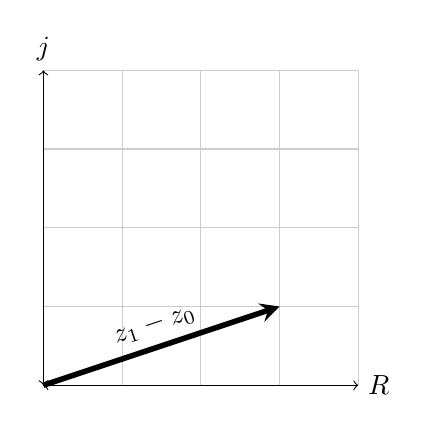
\begin{tikzpicture}
    \draw [thin,gray!40] (0,0) grid (4,4);
    \draw[<->] (0,0)--(4,0) node[right] {$R$};
    \draw[<->] (0,0)--(0,4) node[above]{$j$};
    \draw[line width=2pt,black,-stealth] (0,0)--(3,1) node[midway, above, sloped]{$z_1-z_0$};
\end{tikzpicture}

            \end{minipage}
            \caption{Resta de números complejos}
            \label{fig:RestC}
        \end{figure}
        Entonces restar 2 numero complejos da como resultado un vector de origen en $z_0$ y punto final $z_1$ y también se pude representar como un vector con origen en el punto $(0,j0)$ y final $(x_0-x_1)+j(y_0-y_1)$
    \end{itemize}
\unsubsection{Multiplicación} 
    La multiplicación, al ser el plano complejo un campo vectorial, se computa multiplicando todos los elementos entre ellos y recordando que $j\cdot j=-1$ de la ecuación \ref{eq:jj}. Entonces: 
        \begin{equation}\label{eq:mul}
        \begin{aligned}
            z_1\cdot z_2 \Rightarrow (x_1+y_1j)\cdot(x_2+y_2j)&=(x_1\cdot x_2)+(x_1\cdot y_2j)+(x_2\cdot y_1j)+(y_1j\cdot y_2j)\\
             &=(x_1\cdot x_2)+j^2(y_1\cdot y_2)+j(x_1\cdot y_2+x_2\cdot y_1)\\
             &=(x_1\cdot x_2-y_1\cdot y_2)+j(x_1\cdot y_2+x_2\cdot y_1)
        \end{aligned}
        \end{equation}
    La multiplicación en la forma exponencial es mucho mas simple, recordando la propiedad de la potencia $a^b \cdot a^c=a^{(b+c)}$:
    \begin{equation}\label{eq:mulE}
        z_1\cdot z_2 = r_1e^{j\theta}\cdot r_2e^{j\phi} \lrah z_1\cdot z_2 = (r_1 r_2)e^{j(\theta+\phi)}
    \end{equation}
    Por lo tanto la multiplicación de 2 números complejos da como resultados otro numero complejo, el cual su modulo es la multiplicación de los 2 primeros módulos y su argumento es la suma de los argumentos de los factores. Con este concepto es trivial desarrollar la multiplicación en forma polar, ya que tenemos todos los datos necesrios.
    \begin{equation*}
         z_1\cdot z_2=r_1[\cos{\theta}+j\sin{\theta}]\cdot r_2[\cos{\phi}+j\sin{\phi}]
    \end{equation*}
    \begin{equation}
        z_1\cdot z_2 =(r_1\cdot r_2)[\cos{(\theta +\phi)}+j \sin{(\theta +\phi})]
    \end{equation}
    De aquí se puede intuir que el elemento neutro de la multiplicación es aquel numero complejo que tenga modulo igual a $1$ y argumento igual a $0$:
    \begin{equation}
        z_1\cdot z_n = r_1e^{j\theta}\cdot 1e^{j0} \Longrightarrow z_1\cdot z_n = (r_1 1)e^{j(\theta+0)}
    \end{equation}
    A través de la ecuación \ref{eq:defPol} podemos encontrar que:
    \begin{equation}
        z_n = 1\cdot[\cos{(0)}+j\sen{(0)}] = (1\ ,\ j0)
    \end{equation}
    Por lo tanto el elemento neutro de la multiplicación es el versor $(1\ ,\ j0)$, que es la unidad real.
    
    Un caso que cabe resaltar es la multiplicación por la unidad imaginaria $j$. Como se puede demostrar, la unidad imaginaria tiene un modulo igual a $1$ y argumento igual a $90^{\circ}$ o lo que viene siendo lo mismo $\pi/2$ radianes:
    \begin{equation}
        z_1\cdot j = r_1e^{j\theta}\cdot 1e^{j\frac{\pi}{2}} \Longrightarrow z_1\cdot j = (r_1 1)e^{j(\theta+\frac{\pi}{2})}
    \end{equation}
    o en cartesianas
    \begin{equation}
        z_1\cdot j = (a\ , \ jb)\cdot j \Longrightarrow (a\cdot j\ ,\ j\cdot jb)=(-b\ ,\ ja)
    \end{equation}
   Como se pude apreciar, multiplicar cualquier numero complejo por $j$ da como resultado el mismo vector rotado $90^{\circ}$
   \begin{figure}[H]
       \centering
       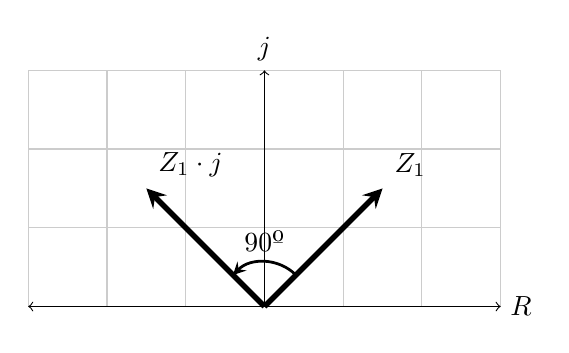
\begin{tikzpicture}
        \draw[thin,gray!40] (-3,0) grid (3,3);
        \draw[<->] (-3,0)--(3,0) node[right] {$R$};
        \draw[<->] (0,0)--(0,3) node[above]{$j$};
        \draw[line width=2pt,black,-stealth](0,0)--(1.5,1.5) node[anchor=south west]{$Z_1$};
        \draw[line width=2pt,black,-stealth](0,0)--(-1.5,1.5) node[anchor=south west]{$Z_1\cdot j$};
        \draw[line width=1pt,black,-stealth] (0.4,0.4) arc (45:135:0.566) node[midway, above]{90º};
\end{tikzpicture}
\caption{Numero complejo multiplicado por la unidad imaginaria}
       \label{fig:MultiC}
   \end{figure}
    Otro caso interesante en el análisis es el caso de multiplicar a un $z_1=(a\ ,\ jb)$ por $z_2=(a\ ,\ -jb)$:
    \begin{equation}
    \begin{aligned}
        z_1\cdot z_2 \Rightarrow (a+jb)\cdot(a-jb)&=(a\cdot a)+(a\cdot jb)+(a\cdot -jb)+(jb\cdot -jb)\\
             &=a^2+j^2(b\cdot -b)+j(a\cdot b-a\cdot b)\\
             &=a^2+b^2
    \end{aligned}
    \end{equation}
    El resultado de esta multiplicación nos da un numero completamente real, que es igual al cuadrado del modulo de $z$. Por esta propiedad a $z_2$ se le suele llamar el conjugado de $z_1$. El conjugado ($z^*$) de un numero complejo es, entonces, otro numero complejo con igual parte real y opuesta parte imaginaria, esto se puede pensar como una reflexión con respecto al eje real.
    \begin{figure}[H]
        \centering
        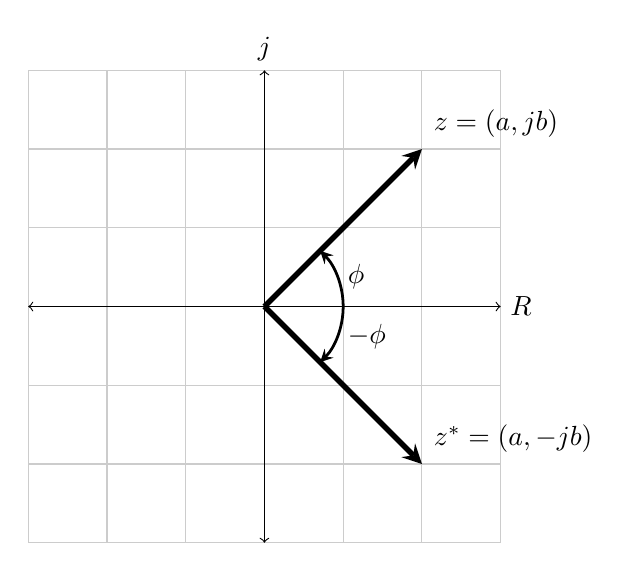
\begin{tikzpicture}
        \draw[thin,gray!40] (-3,-3) grid (3,3);
        \draw[<->] (-3,0)--(3,0) node[right] {$R$};
        \draw[<->] (0,-3)--(0,3) node[above]{$j$};
       \draw[line width=2pt,black,-stealth](0,0)--(2,2) node[anchor=south west]{${z=(a,jb)}$};
       \draw[line width=2pt,black,-stealth](0,0)--(2,-2) node[anchor=south west]{${z^*=(a,-jb)}$};
       \draw[line width=1pt,black,-stealth] (1,0) arc (0:45:1) node [midway, right]{$\phi$};
        \draw[line width=1pt,black,-stealth] (1,0) arc (0:-45:1) node [midway, right]{$-\phi$};
    \end{tikzpicture}
    \caption{conjugado de un numero complejo}
        \label{fig:ConjC}
    \end{figure}
    Como se deja intuir en la figura \ref{fig:ConjC}, en su forma exponencial o polar, el conjugado de $z$ es otro numero complejo de igual modulo y argumento opuesto.
    \begin{equation}
       z= re^{j\phi} \lrah z^*= re^{-j\phi}
    \end{equation}
    Enumerando las propiedades de la multiplicación 
\begin{itemize}
    \item Conmutatividad:
        \begin{equation}
            (a\ ,\ jb)\cdot(\hat{a}\ ,\ j\hat{b})=(\hat{a}\ ,\ j\hat{b})\cdot(a\ ,\ jb)
        \end{equation}
    \item Asociatividad:
        \begin{equation}
            [(a\ ,\ jb)\cdot(\hat{a}\ ,\ j\hat{b})]\cdot(\bar{a}\ ,\ j\bar{b})=(a\ ,\ jb)\cdot[(\hat{a}\ ,\ j\hat{b})\cdot(\bar{a}\ ,\ j\bar{b})]
        \end{equation}
    \item Distributiva:
    \begin{equation}
        (a\ ,\ jb)\cdot((\hat{a}\ ,\ j\hat{b})+\lambda)=  (a\ ,\ jb)\cdot(\hat{a}\ ,\ j\hat{b})+\lambda \cdot (a\ ,\ jb)
    \end{equation}
    \item Elemento neutro:
        \begin{equation}
             (a\ ,\ jb)\cdot(1\ ,\ j0) \lrah (a\cdot 1 + \bcancel{a\cdot j0}) +\ (jb\cdot 1+\bcancel{jb\cdot j0}))=a+jb 
        \end{equation}
    \item Inverso: 
    En esta propiedad nos vamos a detener ya que no es trivial el análisis.
    La inversa de la multiplicación es la división, que es $z_1/z_2$ también se pude escribir como $z_1\cdot z_2^{-1}$ nos faltaría definir como se computa el inverso de un numero complejo:
    \begin{equation*}
        \cfrac{1}{z}=\cfrac{1}{a+jb} \lrah \cfrac{1}{a+jb}\cdot\cfrac{a-jb}{a-jb}=\cfrac{a-jb}{a^2+b^2}
    \end{equation*}
    \begin{equation}
        \cfrac{1}{z}=\cfrac{a}{a^2+b^2}-j\cfrac{b}{a^2+b^2}
    \end{equation}
    Es necesario recalcar que se multiplica $1/z$ por $z^*/z^*$ para eliminar la parte imaginaria del denominador.
    
    Se pude probar lo mismo de manera mas sencilla representando a $z$ en su forma exponencial y recordando la propiedad$1/a^x=a^{-x}$:
    \begin{equation}
        \cfrac{1}{z}=\cfrac{1}{re^{j\theta}} \lrah \cfrac{1}{z}=\cfrac{1}{r}e^{-j\theta}
    \end{equation}
    Entonces el inverso de un numero complejo da como resultado otro numero complejo de modulo $1/r$ y argumento $-\theta$.
    Con esto explicado podemos razonar que  dividir un $z_1$ por un $z_2$ no es mas que multiplicar $z_1$ por el inverso de $z_2$:
    \begin{equation}
        \cfrac{z_1}{z_2}= r_1e^{j\theta}\cdot \cfrac{1}{r_2}e^{-j\phi} \lrah 
        \begin{cases}
            \cfrac{z_1}{z_2} = (\cfrac{r_1}{r_2})e^{j(\theta-\phi)}\\
            \\
            \cfrac{z_1}{z_2} =(\cfrac{r_1}{r_2})[\cos{(\theta -\phi)}+j \sin{(\theta -\phi})] 
        \end{cases}
    \end{equation}
    
    Si multiplicamos a un $z$ por $1/z$ obtendremos el elemento neutro de la multiplicación:
     \begin{equation}
        z\cdot \cfrac{1}{z}=re^{(j\theta)}\cfrac{1}{re^{j\theta}} \lrah \cfrac{z}{z}=\bcancel{\cfrac{r}{r}}e^{\bcancel{j\theta-j\theta}} = 1e^{j0} = (1,j0)
    \end{equation}
    
    \end{itemize}
\unsubsection{Potenciación} 
    La potenciación de un numero $z$ en $n$ no es mas que la multiplicación sucesiva de $z$ $n$ veces. Se recomienda computar la potenciación en la forma polar o exponencial:
    \begin{equation}\label{eq:defPot}
        z^n=\begin{cases}
        (re^{j\theta})^n \lrah z^n =r^ne^{j\theta \cdot n} \\
        \\
        (r[\cos{(\theta)}+j\sin{(\theta)}])^n \lrah z^n = (r^n)[\cos{(\theta \cdot n)}+j \sin{(\theta \cdot n})]
        \end{cases}
    \end{equation}
    En términos de propiedades es distributiva en la multiplicación:
    \begin{equation}
        ((a\ ,\ jb)\cdot \lambda)^n = (a\ ,\ jb)^n\cdot \lambda^n
    \end{equation}
    Y elevar cualquier numero imaginario por $0$ da como resultado la unidad real, partiendo de \ref{eq:defPot}:
    \begin{equation}
        z^0=(r^0)[\cos{(\theta \cdot 0)}+j \bcancel{\sin{(\theta \cdot 0}})] = 1\cdot[1+j0] = (1\ ,\ j0)
    \end{equation}
\unsubsection{Radicación}
    La radicación es un poco mas compleja que la potenciación, se recomienda ver la unidad de funciones complejas y mapeo antes de ver este tema.
    Se debe recordar que los números complejos son periódicos en $2\pi$ por lo tanto y haciendo uso de la ecuación \ref{eq:defPol} se puede escribir un numero complejo de la siguiente manera:
    \begin{equation}
        z = r[\cos{(\theta + 2\pi k)}+j\sin{(\theta + 2\pi k)}] \llrah \ z = re^{j(\theta+2\pi k)}
    \end{equation}
    $k$ siendo cualquier numero entero.
    Esto es necesario ya que la raíz tiene múltiples respuestas a un mismo numero complejo ya que afecta el carácter periódico de la misma. Recordando que la raíz enésima se puede expresar como $\sqrt[n]{a}=a^{1/n}$ y la definición de la potenciación \ref{eq:defPot}:
    \begin{equation}\label{eq:defRad}
        z^{\frac{1}{n}} = (re^{j(\theta+2\pi k)})^{\frac{1}{n}}
        \begin{cases}
             z^{\frac{1}{n}} = r^{\frac{1}{n}}e^{j(\frac{\theta+2\pi k}{n})}\\
             \\
             z^{\frac{1}{n}} = r^{\frac{1}{n}}[\cos{(\frac{\theta + 2\pi k}{n})}+j\sin{(\frac{\theta + 2\pi k}{n})}]
        \end{cases}
    \end{equation}
    Como se pude apreciar la radicación de un numero complejo da otro numero complejo de modulo $r^{(1/n)}$, pero lo interesante pasa por ver que le sucede al argumento.
    Ahora el argumento esta dado por la expresión $\frac{\theta + 2\pi k}{n}$ que la podemos descomponer en dos partes, $\frac{\theta}{n}$ y $\frac{2\pi k}{n}$, recordemos que $n$ es una constante y $k$ una variable que solo puede tomar valores de números enteros. La segunda expresión le da el carácter periódico al numero complejo pero esta expresión dejo de ser igual a un múltiplo de $2\pi$, para que este vuelva a ser el caso $k$ debe ser igual a $\lambda \cdot n$, $\lambda$ siendo un numero entero.
    \begin{equation*}
        \cfrac{2\pi k}{n}
        \begin{cases}
            k=\lambda n \lrah \cfrac{2\pi k}{n} =  2\pi \lambda \\
            \\
            k \neq \lambda \lrah \cfrac{2\pi k}{n}
        \end{cases}
    \end{equation*}
    Por lo tanto existen $n$ distintos argumentos que no se repiten en $2\pi$.
    
    Tomando en cuenta esto existen $n$ respuestas a la raíz enésima de un numero complejo:
    \begin{equation}
    \begin{aligned}
         z^{\frac{1}{n}}= & r^{\frac{1}{n}}[\cos{(\frac{\theta + 2\pi \cdot 0}{n})}+j\sin{(\frac{\theta + 2\pi \cdot 0}{n})}]\\
                        & r^{\frac{1}{n}}[\cos{(\frac{\theta}{n} +\frac{2\pi \cdot 1}{n})}+j\sin{(\frac{\theta}{n} +\frac{2\pi \cdot 1}{n})}]\\
                        & r^{\frac{1}{n}}[\cos{(\frac{\theta}{n} +\frac{2\pi \cdot 2}{n})}+j\sin{(\frac{\theta}{n} +\frac{2\pi \cdot 2}{n})}]\\
                        & r^{\frac{1}{n}}[\cos{(\frac{\theta}{n} +\frac{2\pi \cdot 3}{n})}+j\sin{(\frac{\theta}{n} +\frac{2\pi \cdot 3}{n})}]\\
                        &\hspace{3.6cm} \cdot \\
                        &\hspace{3.6cm} \cdot \\
                        &\hspace{3.6cm} \cdot \\
                        &\hspace{3.37cm} \ldots \\
                        & r^{\frac{1}{n}}[\cos{(\frac{\theta}{n} +\frac{2\pi \cdot (n-2)}{n})}+j\sin{(\frac{\theta}{n} +\frac{2\pi \cdot (n-2)}{n})}]\\
                        & r^{\frac{1}{n}}[\cos{(\frac{\theta}{n} +\frac{2\pi \cdot (n-1)}{n})}+j\sin{(\frac{\theta}{n} +\frac{2\pi \cdot (n-1)}{n})}]\\
    \end{aligned}
    \end{equation}
    Planteando el ejemplo de numero complejo $(\-0.5735,\ j0.819)$:
    \begin{enumerate}
        \item Obtenemos la expresión en la forma polar, para este caso este numero tiene un modulo de $1$ y un argumento de $125^{\circ}$ que equivalen a $\frac{25}{36}\pi$ radianes:
        \begin{equation}
         z= 1e^{j\pi(\frac{25}{36}+2k)} \llrah z = 1[\cos{(125^{\circ} + 360^{\circ} k)}+j\sin{(125^{\circ} + 360^{\circ} k)}]
        \end{equation}
        \item Planteamos una radicación de orden 5 por ejemplo, recordando la definición de radicación \ref{eq:defRad}:
        \begin{equation}
            \sqrt[5]{z}=\sqrt[5]{1} \cdot [\cos{\frac{(125^{\circ} + 360^{\circ} k)}{5}}+j\sin{\frac{(125^{\circ} + 360^{\circ}}{5} k)}]
        \end{equation}
        \begin{equation}\label{eq:RadCej} 
            \sqrt[5]{z}=1[\cos{(25^{\circ} + 72^{\circ} k)}+j\sin{(25^{\circ} + 72^{\circ}k)}]
        \end{equation}
        Podemos ver que el argumento de las raices van a variar en $72^{\circ}$ uno del otro y que solo nos hace falta valuar $0\leqslant k \leqslant 4$ ya que cunado $k=5$ lo que suma a los $25^{\circ}$ va a ser igual a $360^{\circ}$ o 
 $2\pi$ radianes y se van a empezar a repetir los argumentos.
    \end{enumerate}
\begin{figure}[H]
    \centering
    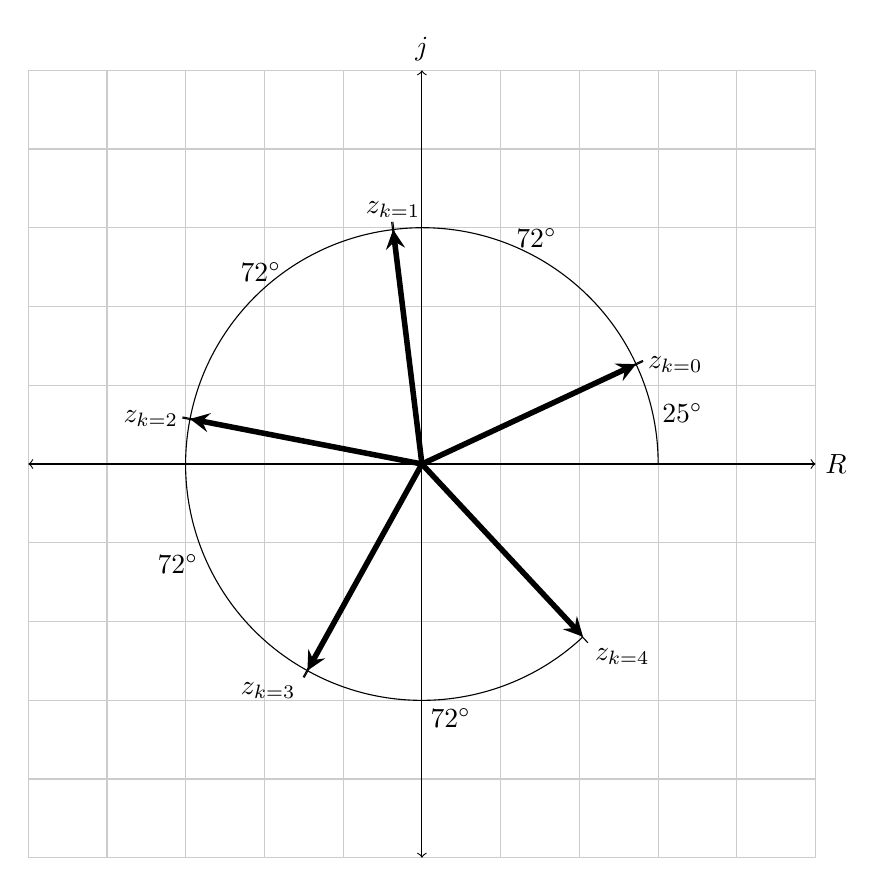
\begin{tikzpicture}
        \draw[thin,gray!40] (-5,-5) grid (5,5);
        \draw[<->] (-5,0)--(5,0) node[right] {$R$};
        \draw[<->] (0,-5)--(0,5) node[above]{$j$};
        \draw[line width=2pt,black,-stealth](0,0)--(2.72,1.268) node[right]{${z_{k=0}}$};
        \draw[line width=2pt,black,-stealth](0,0)--(-0.3656,2.977) node[above]{${z_{k=1}}$};
        \draw[line width=2pt,black,-stealth](0,0)--(-2.945,0.5724) node[left]{${z_{k=2}}$};
        \draw[line width=2pt,black,-stealth](0,0)--(-1.4544,-2.624) node[anchor=north east]{${z_{k=3}}$};
        \draw[line width=2pt,black,-stealth](0,0)--(2.046,-2.194) node[anchor=north west]{${z_{k=4}}$};
        \draw[|-|] (3,0) arc (0:25:3) node [midway, right]{$25^{\circ}$};
        \draw[|-|] (2.72,1.268) arc (25:97:3) node [midway,above]{$72^{\circ}$};
        \draw[|-|] (-0.3656,2.977) arc (97:169:3) node [midway, above]{$72^{\circ}$};
        \draw[|-|] (-2.945,0.5724) arc (169:241:3) node [midway, left]{$72^{\circ}$};
        \draw[|-|] (-1.4544,-2.624) arc (241:313:3) node [midway, below]{$72^{\circ}$};
    \end{tikzpicture}
    \caption{Representación de la ecuación \ref{eq:RadCej} en el intervalo marcado}
    \label{fig:RadC}
\end{figure}
\unsubsection{Logaritmo natural}
El logaritmo natural de un numero complejo es la inversa de la forma exponencial. La única forma de computar el logaritmo natural cómodamente es con la forma exponencial del numero. Recordando la propiedades de los logaritmos $\ln{(e)}=1$, $\ln{(a\cdot b)}=\ln{(a)}+\ln{(b)}$ y $\ln{(a^b)}=b\cdot \ln{(a)}$:
\begin{equation} \label{eq:defLnC}
    \ln{z}=\ln{(re^{j\theta})}\lrah \ln{z}=\ln{(r)}+j\theta
\end{equation}
Como vemos en la ecuación \ref{eq:defLnC} el logaritmo natural de un numero complejo, en su forma exponencial, da como resultado un otro numero complejo en forma cartesiana de parte real igual al logaritmo natural del radio y parte imaginaria igual a su argumento.
\unsection{Otros operadores}
Para los números complejos existen otras operaciones exclusivas que son útiles en el analisis complejo.
\begin{itemize}
    \item Operador $\Real{}$:
    Este operador devuelve la parte real de un numero complejo y descarta la parte imaginaria.
    \begin{equation}\label{eq:DefImagC}
        z=(a+jb) \lrah \Real{z}=a
    \end{equation}
     \item Operador $\Imag{}$: 
     Similar al operador $\Real{}$, este operador toma la parte imaginaria de un numero complejo y descarta la parte real
     \begin{equation}\label{eq:DefRealC}
         z=(a+jb) \lrah \Imag{z}=b
     \end{equation}
     \item Operador $*$:
      Aunque ya hayamos presentado el concepto de números conjugados, formalmente $*$ es un operador que devuelve el conjugado de un numero complejo.
      \begin{equation}\label{eq:DefConC}
          z=(a+jb) \lrah z^*=(a-jb)
      \end{equation}
      \item Operador modulo $||$:
      Este operador devuelve el modulo de un numero complejo:
      \begin{equation}\label{eq:DefModC}
          |z|=\sqrt{x^2+y^2} \llrah\ |z|=|re^{j\theta}|=r \llrah\ |z|=|r[\cos{\theta}+j\sin{\theta}]|=r
      \end{equation}
      Cuando el numero $z$ es escalado un $\lambda$ entonces el modulo estará multiplicado por $\lambda$:
      \begin{equation}
          |\lambda z|=\sqrt{(\lambda x)^2+(\lambda y)^2}\lrah\sqrt{\lambda^2(x^2+y^2)}=\lambda\sqrt{x^2+y^2}
      \end{equation}
      \begin{equation}
          |\lambda z|=\lambda|z|
      \end{equation}
      \item Operador $Arg$ o $\angle$:
      Este operador devuelve el argumento del modulo, siendo $z=x+jy$:
      \begin{equation}
          Arg(z)=\tan^{-1}{(\frac{y}{x})} \llrah\ Arg(re^{j\theta})=\angle\theta \llrah\ Arg(r[\cos{\theta}+j\sin{\theta}])=\angle\theta
      \end{equation}
      
     
\end{itemize}